% Font size, paper type
\documentclass[12pt]{article}
% Aesthetic margins
\usepackage[margin=1in]{geometry}
% Core math packages,
% Mathtools loads amsmath, and amsmath gives basic math symbs
% Amsfonts & amssymb are misc. symbols you might need
\usepackage{mathtools, amsfonts, amssymb}
% Links in a pdf
\usepackage{hyperref}
% Hex values for colors; custom colors
\usepackage{xcolor}
% Use in pictures, graphs, and figures
\usepackage{graphicx}
% Header package
\usepackage{fancyhdr}
% Underlining with line breaks
\usepackage{ulem}
% Adjust accordingly given warning messages
\setlength{\headheight}{15pt}
% So we can more easily format text with pictures
\usepackage{float}
% Images and drawing graphs
\usepackage{tikz}
% Something about bits and stuff
\usepackage[T1]{fontenc}
% Set the incoding to unicode instead of ascii
\usepackage[utf8]{inputenc}
% Set the font to arial
% \usepackage{fontspec}
% \usepackage{mathspec}
% \setmainfont{Arial}
% \setmathrm{Arial}
% \setmathfont(Digits,Latin){Arial}
% Defines stuff about tables
\usepackage{tabularx}
% Similar to `lorem*[n]` in emmet
\usepackage{lipsum}
% Spits columns into two, the sane way
\usepackage{paracol}
% Layout of two columns
% \usepackage{multicol}
% Removes automatic indent at the start of a paragraph
\usepackage{indentfirst} 
% Modularity! Includes other .tex files, precompiled
% Use \subfile{path_of_doc} to include other filesr
\usepackage{subfiles}

% Sets footer
\pagestyle{fancy}
% Removes default footer style
\fancyhf{}

\rhead{\thepage{}}

% Makes links look more appealing
\hypersetup{ 
colorlinks=true,
% linkcolor=blue,
% filecolor=magenta,
% urlcolor=blue,
}

\begin{document}
\title{Noise Cancellation}
\author{by Shengdong Li}
\date{26 October 2021}
\maketitle

\section{Research Question}

How does the difference in phase between two waves affect the sound level at a certain point between them?

\section{Background}

\subsection{Wave Interference}

The superpositioning of two waves which are in phase with each other causes destructive or constructive interference depending on the position. Perfect constructive interference is when the two waves match up directly, thus causing the amplitude to double. Conversely, when the two waves are exactly \(\frac{1}{2}\lambda\) apart, perfect destructive interference occurs, such that the amplitude of the two waves equals zero.

...

\subsection{Sound Intensity}

The sound intensity of a wave depends both on the energy of the wave and the area in which it travels through, and "it's related to" the "amplitude squared" of the sound wave.

...

\subsection{Sound Level}

Humans don't react to sound intensity at a linear level. Instead, it's more of an exponential relationship. Decibels factor this in, as louder sounds need exponentially more energy in order to sound "louder" to humans.

...

\section{Hypothesis}

The difference in displacement between two in-phase waves would have a sinusoidal relationship with the sound intensity level, due to constructive and destructive interference causing cyclic patterns of change in amplitude of the resulting sound.

\subsection{Prediction Graph (remove later)}


\begin{figure}[H]
    \centering
    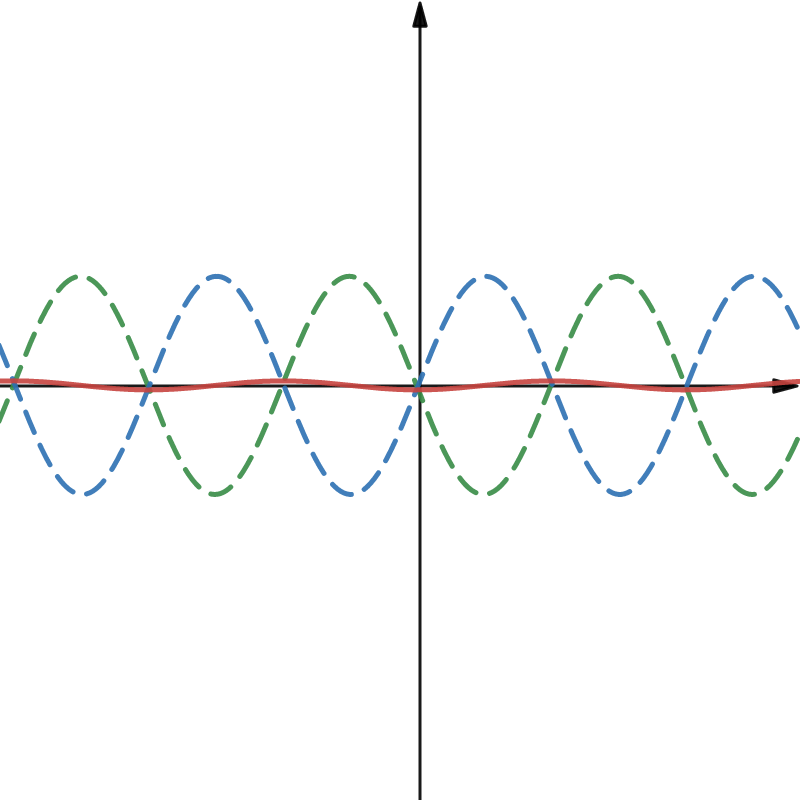
\includegraphics[scale=0.3]{prediction.png}
    \caption{Predicted graph. Red line is the resulting amplitude. \href{https://www.desmos.com/calculator/ahmohu46il}{link}}
\end{figure}

\section{Variables and Explanations}

\subsection{Independent Variable}

The independent variable in this case would be the phase-shifted distance between the two waves. Its units would be in meters. It will be set by varying the start time that noise is emitted between on speaker and the other, via a computer program. This time will be multiplied with the speed of sound constant to calculate the distance the two waves are shifted.

The uncertainty in this case would be because of variation of time that it takes for the cpu to run a specific program, which would nearly be negligible and nearly impossible to calculate.

\subsection{Dependent Variable}

The sound level will be the dependent variable of the equation. It will be in the units of decibel. This measurement will be taken with the microphone on a used samsung galaxy sx running the recording app xxx, for ten seconds. Then samples will be taken every second and averaged. The uncertainty here will arise from the sensitivity of the microphone.

\subsection{Controlled Variable}

\textbf{The position of the microphone} should be kept constant at every trial. This is because while for perfect destructive interference the amplitude of the wave everywhere would be zero, because sound waves are sinusoidal their amplitudes differ at certain points. A distance further away from the source would also result in decreasing sound levels due to the fact that energy travels away in a sphere so much of it is lost to the environment further out.

\textbf{The frequency and wavelength of the two waves} The frequency of two waves should be kept the exact same. In order for perfect constructive and destructive interference to occur, the two waves must be perfectly in-phase with each other, otherwise the resulting wave would be very uneven and there would be varying results everytime.

\textbf{The temperature of the room} The temperature of the room should be kept constant because temperatureand movement of particles in the air affects the amount of energy lost as the wave propogates forward.

\textbf{Ambient Sound Level} The ambient sound level should be kept constant because otherwise the dependent variable of sound level would be modified not just by the independent variable but also by the environment, which would invalidate the experiment.

\section{Method}

\begin{figure}[H]
    \centering
    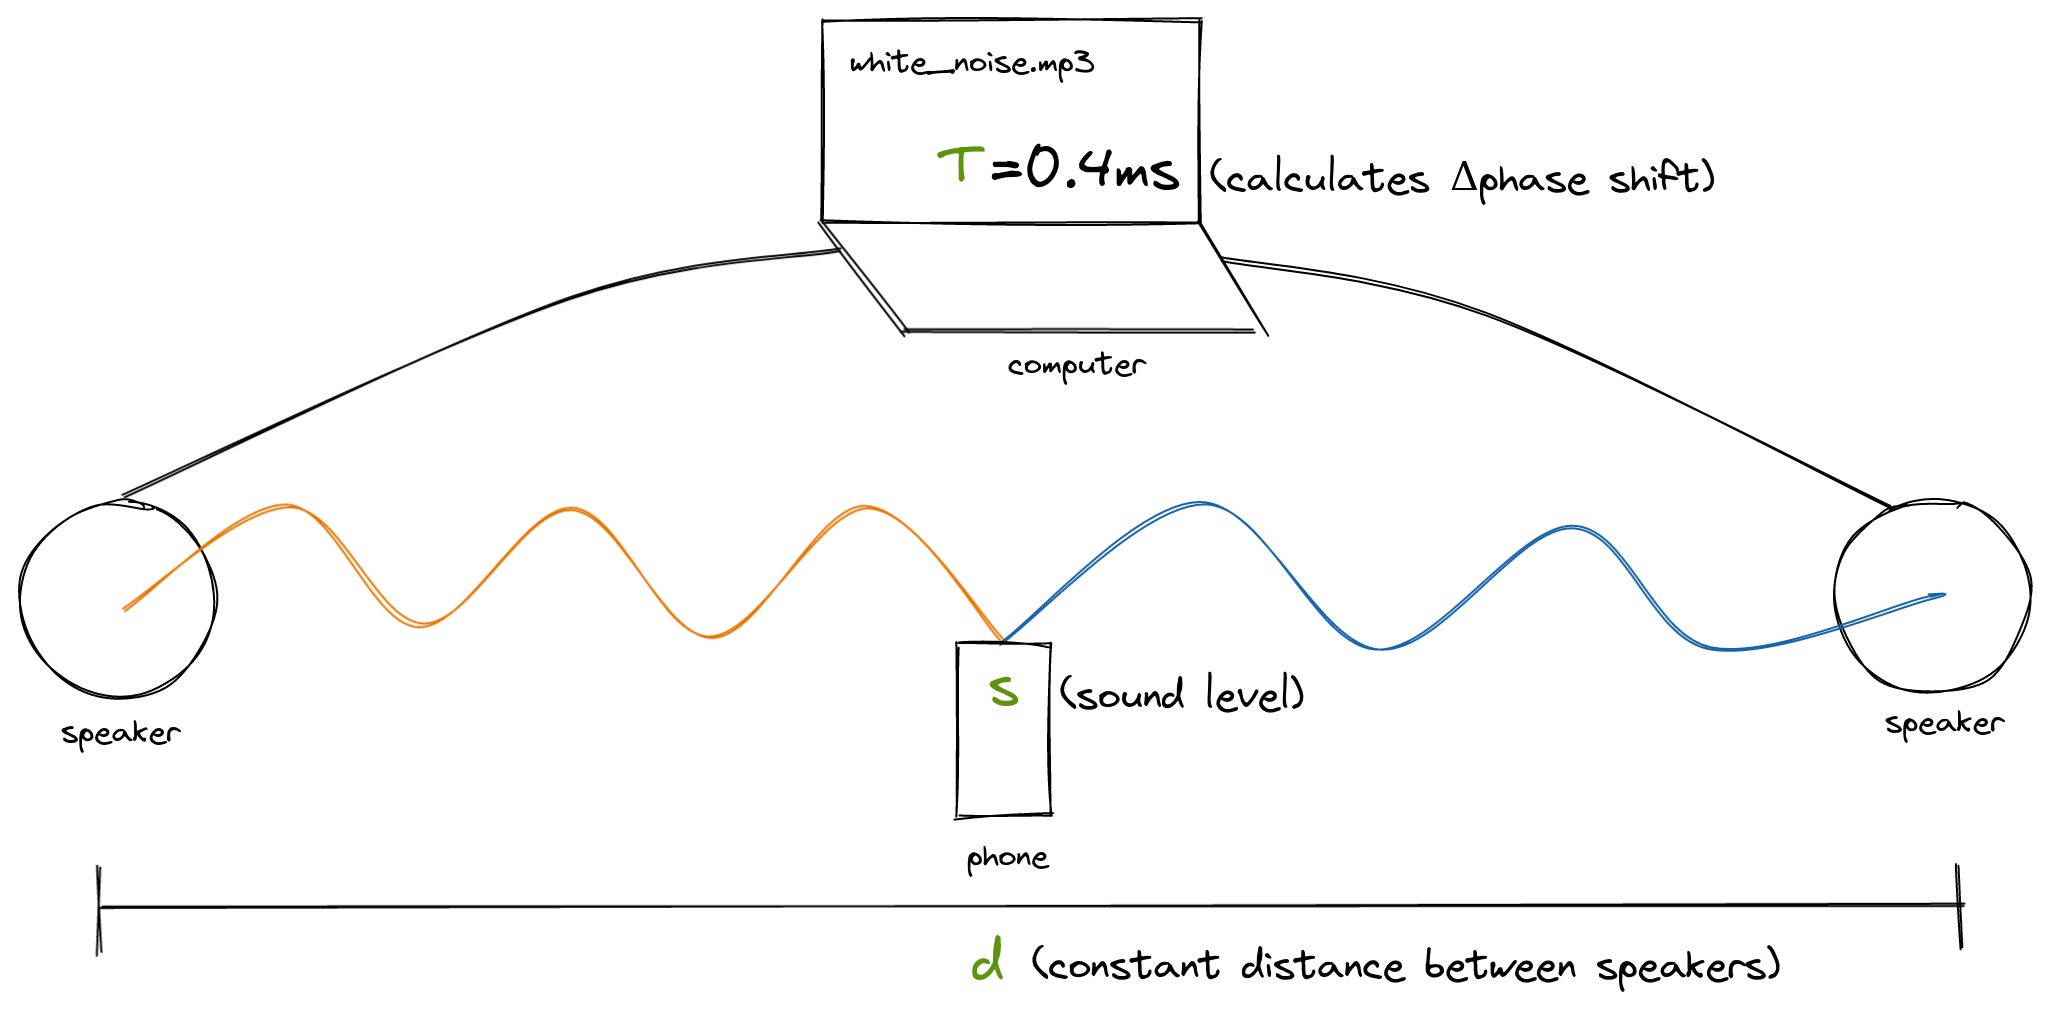
\includegraphics[scale=0.24]{sound_diagram.png}
    \caption{Sketch of experiment setup.}
\end{figure}

\begin{enumerate}
    \item Position two identical speakers around 5 meters apart from each other
    \item Connect the speakers to a computer
    \item Put a phone face up between the middle of the two speakers
    \item Run a computer program that plays a monotone sound through one speaker, then powers on the other speaker 1 millisecond after the other speaker.
    \item With the speakers playing, begin recording audio on the phone for 10 seconds, trimming out the empty audio at the start and the end
    \item Take samples at every second from 0 seconds to 10 seconds, then average these 11 samples into one and record this data point
    \item Repeat sampling 3 times
    \item Repeat the entire thing with 1, 2, 3, 4, 5 millisecond delays
\end{enumerate}

\subsection{Safety}

Safety precautions should be made to ensure that the speaker sound levels do not go above maximal decibel sound levels that humans are tolerant of, to preserve the health of the ear.

\section{Evaluation and Discussion}???

\subsection{Strengths}

The use of a computer to change the independent variable, change in phase between two identical waves, offers a very high degree of accuracy, especially in dealing with waves travelling at the speed of light. This should result in a very low degree of uncertainty in the measurement of the independent variable.

The fact that this test includes mostly electronics allows for easy automation of collected data. This results in data being collected in a smaller time frame, which minimizes the impact that the environment, in ambient noise level and temperature.

\subsection{Weaknesses}

It's hard to do the experiment outside, because there are no plugs outside. Therefore, when doing the experiment inside, reverb from walls may cause sound distortions that affect sound levels in unforseen ways, for example, waves may bounce off from the left and right instead of head on and collide fourway in the middle, exacerbating maximum amplitudes and increasing the deviation of data.

To prevent this, sound dampeners may be placed on the side of the wall, for example blankets.

\section{Works Cited}

Urone, P. P., \& Hinrichs, R. (2012). Superposition and Interference. In \textit{College Physics}. OpenStax. https://openstax.org/books/college-physics/pages/16-10-superposition-and-interference

\end{document}
